\section{Calibration and Monte Carlo Simulation}\label{sec:simulation}

% Role: quantifies the offset ratio Omega (def:offset) for the US and Europe; all values come from code, never typed by hand.

\subsection{Calibration}\label{sec:sim-calibration}

We calibrate the baseline model of \cref{sec:theory} to match US business dynamism moments from the Business Dynamics Statistics (BDS).
The span-of-control parameter $\alpha = 0.64$ follows \citet{hopenhayn1993job}; this implies a displacement threshold $\theta = 1/(1-\alpha) \approx 2.78$.
Entry and fixed costs are set to match pre-2020 entry and exit rates of approximately 7--8\%.
The productivity process targets the right-skewed firm size distribution documented by \citet{axtell2001zipf}.

For the AI shock, we treat the key parameters as uncertain and draw them from prior distributions rather than calibrating to point estimates, since AI diffusion is ongoing and the relevant elasticities are not yet well identified.

\begin{table}[t]
  \centering
  \caption{Calibration}
  \label{tab:calibration}
  \begin{tabular}{llcl}
    \toprule
    Parameter & Description & Value & Target or source \\
    \midrule
    $\alpha$ & Returns to scale & 0.64 & \citet{hopenhayn1993job} \\
    $\beta$ & Discount factor & 0.96 & Standard annual \\
    $c_e$ & Entry cost (pre-AI) & 20 & Entry rate $\approx 7\%$ \\
    $c_f$ & Fixed operating cost & 0.5 & Exit rate $\approx 7\%$ \\
    $\rho$ & Productivity persistence & 0.97 & Size distribution \\
    $\sigma_z$ & Productivity shock s.d. & 0.18 & \citet{axtell2001zipf} \\
    \midrule
    \multicolumn{4}{l}{\textit{AI shock parameters (Monte Carlo priors)}} \\
    $\sigma_{\text{ai}}$ & Labor-AI substitution & $\mathcal{U}(2, 5)$ & Spans threshold \\
    $1-\kappa_e$ & Entry cost reduction & $\mathcal{U}(0, 0.30)$ & Cloud-era range \\
    $\Delta \mu_e$ & Entrant productivity shift & $\mathcal{U}(0, 0.15)$ & AI-native advantage \\
    $F_{\text{ai}}$ & AI adoption fixed cost & $\mathcal{U}(2, 10)$ & Size-selective adoption \\
    \bottomrule
  \end{tabular}
\end{table}

\subsection{Monte Carlo design}\label{sec:sim-design}

Because the parameters of the AI shock are uncertain, we use the CES specification of \cref{sec:ai-ces} and treat the shock vector $\Phi = (\sigma_{\text{ai}}, \kappa_e, \Delta\mu_e, F_{\text{ai}})$ as random rather than calibrated to a point.
The four components are drawn independently; the fixed operating cost is held at its pre-shock value ($\kappa_f = 1$), as are the price of AI services and the relative AI exposure of each sector.
For each draw $\Phi^{(s)}$, $s = 1, \dots, S$, from the prior distribution in \cref{tab:calibration}, we simulate the economy for 40 periods (AI diffuses from period 5) and compute outcomes, averaged over the last 10 periods, by comparing to a no-AI counterfactual from the same initial conditions and random-number seed.
This common-random-numbers design isolates the effect of AI from simulation noise.

The offset ratio $\Omega$ is defined only when large-firm employment falls.
Our headline statistic is therefore the probability that AI raises net employment relative to the counterfactual,
\begin{equation}\label{eq:offset-probability}
  \Pr\bigl[ \Delta N > 0 \bigr] \approx \frac{1}{S} \sum_{s=1}^{S} \mathbf{1}\bigl\{ \Delta N(\Phi^{(s)}) > 0 \bigr\}.
\end{equation}
In draws where large-firm employment falls, $\Delta N > 0$ is the same event as $\Omega \ge 1$, so the probability of offset conditional on large-firm employment falling is the Monte Carlo counterpart to $\Pr[\Omega \ge 1]$.
We also report the distribution of the net employment effect $\Delta N / N_{\text{cf}}$ and its sensitivity to each component of $\Phi$.
We run $S = 2{,}000$ replications (seed 2026), plus 60 fixed-parameter replications to measure pure simulation noise.

\paragraph{Size classes in the simulation.}
The model economy has about 175,000 workers and holds too few firms above 5,000 employees to measure the classes of \cref{sec:theory-equilibrium} reliably.
The simulation therefore uses smaller cutoffs---small (fewer than 20 employees), mid-sized (20 to 499), and large (500 or more)---so that $\Omega$ compares employment at firms below 500 employees with employment at firms of 500 or more.
Firms are classified by current rather than pre-shock size, so the simulated $\Omega$ approximates the cohort-based definition in \cref{def:offset}: a firm that grows across a cutoff counts as a loss in one class and a gain in another.

\subsection{Results}\label{sec:sim-results}

\paragraph{Headline finding: conditional offset.}
\Cref{tab:sim-results} summarizes the outcome probabilities.
Across 2,000 Monte Carlo draws, the probability of net employment offset is 81.7\% (95\% CI: 79.9\%--83.3\%).
The median net employment effect is $+10.6\%$ relative to the no-AI counterfactual, with the 90\% interval spanning $-5.8\%$ to $+51.7\%$.
The probability of strong offset (net employment gain exceeding 5\%) is 66.9\%.

The headline hides an important qualification: \textbf{most of the ``offset'' is absence of displacement, not compensation for it.}
Large-firm (500+ employees) employment falls in only 43.5\% of draws.
Conditional on large-firm employment actually falling, the probability of offset drops to 59.2\% (95\% CI: 55.9\%--62.5\%).

\begin{table}[t]
  \centering
  \caption{Monte Carlo results: probability of offset}
  \label{tab:sim-results}
  \begin{tabular}{lcc}
    \toprule
    Event & Probability & 95\% CI \\
    \midrule
    P(offset): net employment $> 0$ & 81.7\% & [79.9\%, 83.3\%] \\
    P(strong offset): net employment $> 5\%$ & 66.9\% & [64.8\%, 68.9\%] \\
    P(offset $|$ large-firm employment falls) & 59.2\% & [55.9\%, 62.5\%] \\
    P(large-firm employment falls) & 43.5\% & [41.4\%, 45.7\%] \\
    P(concentration): small-firm ($<20$) empl.\ falls & 4.0\% & [3.2\%, 4.9\%] \\
    \bottomrule
  \end{tabular}
\end{table}

\paragraph{What drives the outcome: $\sigma_{\text{ai}}$ dominates.}
The variance decomposition in \cref{tab:sensitivity} shows that the labor-AI substitution elasticity $\sigma_{\text{ai}}$ explains 71\% of the variance in net employment effects (first-order sensitivity index).
The AI entrant productivity shift explains 18\%, while entry-cost reduction explains only 3\%.
The adoption fixed cost has negligible direct effect ($<1\%$).
The ranking differs for small-firm employment, where the entry-side channels matter about as much as $\sigma_{\text{ai}}$ (first-order indices of 31\% for $\sigma_{\text{ai}}$, 30\% for the entrant productivity shift, and 25\% for entry-cost reduction): lower entry costs shape \emph{where} employment sits, but not whether it rises in aggregate.

\begin{table}[t]
  \centering
  \caption{Variance decomposition: what drives net employment?}
  \label{tab:sensitivity}
  \begin{tabular}{lrrr}
    \toprule
    Parameter & Spearman $\rho$ & First-order $S_1$ & Linear $R^2$ share \\
    \midrule
    $\sigma_{\text{ai}}$ (substitution elasticity) & $-0.66$ & 0.71 & 0.45 \\
    $\Delta\mu_e$ (entrant productivity shift) & $+0.53$ & 0.18 & 0.18 \\
    $1-\kappa_e$ (entry cost reduction) & $+0.21$ & 0.03 & 0.02 \\
    $F_{\text{ai}}$ (adoption fixed cost) & $+0.06$ & $<0.01$ & $<0.01$ \\
    \bottomrule
  \end{tabular}
\end{table}

This finding is central to the paper's contribution: \textbf{entry cost reduction, the mechanism most analogous to cloud computing, explains almost none of the variance in employment outcomes.}
What matters is whether AI augments workers ($\sigma_{\text{ai}} < 2.78$) or replaces them ($\sigma_{\text{ai}} > 2.78$), and whether AI-native entrants are more productive than they would have been absent AI.

\paragraph{The role of the displacement threshold.}
Below the threshold $\sigma_{\text{ai}} < 2.78$, the probability of offset is 99.8\% ($n = 547$ draws).
Above the threshold, P(offset) falls to 74.9\% ($n = 1{,}453$).
Even at high substitution elasticities ($\sigma_{\text{ai}} > 4.5$), offset probability remains around 68\%, because higher substitution also reduces AI's cost advantage and hence adoption rates.
\Cref{fig:sigma-threshold} plots the full profile: the threshold marks where offset stops being guaranteed, not a tipping point at which it becomes unlikely.

\begin{figure}[t]
  \centering
  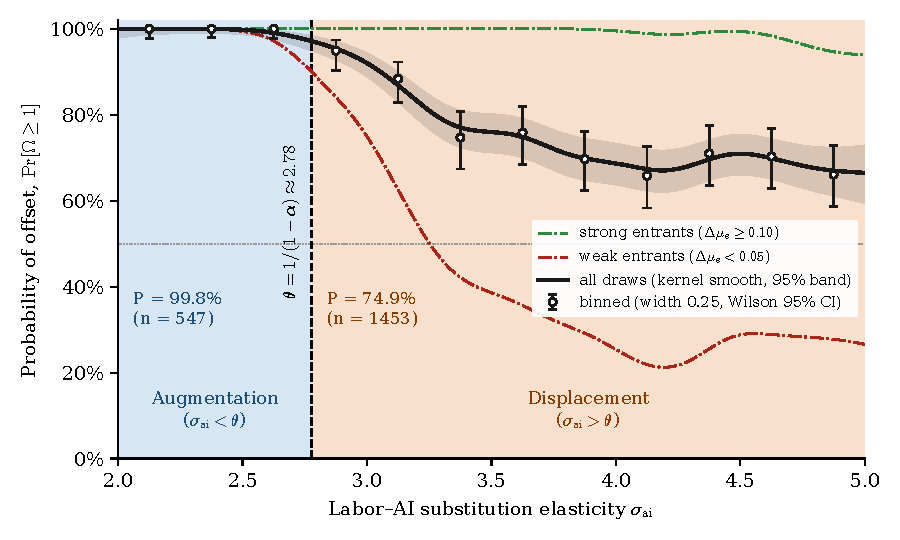
\includegraphics[width=\linewidth]{sigma_threshold}
  \caption{Probability of offset as a function of the labor--AI substitution elasticity.
    Each Monte Carlo draw counts as an offset when the net employment effect is positive. When large-firm (500+) employment falls, this is the same event as $\Omega \ge 1$: gains at firms below 500 employees cover the loss at large firms.
    Points are 0.25-wide bins of $\sigma_{\text{ai}}$ with Wilson 95\% intervals; the solid line is a Gaussian-kernel smooth (bandwidth 0.15) with a 95\% band; dash-dotted lines repeat the smooth for draws with weak ($\Delta\mu_e < 0.05$) and strong ($\Delta\mu_e \ge 0.10$) AI-native entrants.
    The dashed vertical line is the single-firm displacement threshold $\theta = 1/(1-\alpha) \approx 2.78$ (\cref{eq:threshold}).
    In the augmentation region ($\sigma_{\text{ai}} < \theta$) the scale effect dominates, AI raises labor demand at adopting firms, and offset is near-certain (99.8\%, $n = 547$).
    In the displacement region ($\sigma_{\text{ai}} > \theta$) adopters shed workers and offset falls to 74.9\% ($n = 1{,}453$). It levels off near 66--70\% instead of collapsing, because higher $\sigma_{\text{ai}}$ also shrinks AI's cost advantage and so its adoption.
    Above $\theta$, entrant quality decides the outcome: offset stays near 100\% with strong entrants and drops to 20--30\% with weak ones.
    $N = 2{,}000$ draws; data: \texttt{data/monte\_carlo\_raw.csv}; figure: \texttt{scripts/plot\_sigma\_threshold.py}.}
  \label{fig:sigma-threshold}
\end{figure}

The interaction between $\sigma_{\text{ai}}$ and the entrant productivity shift is decisive (\cref{fig:offset-distribution}).
When $\sigma_{\text{ai}} > 3.5$ and the entrant productivity shift is weak ($< 0.05$), P(offset) collapses to 27.8\% ($n = 316$).
When the entrant shift is strong ($\geq 0.10$), P(offset) is 99.3\% pooled across $\sigma_{\text{ai}}$ ($n = 689$), and at least 97\% in every $\sigma_{\text{ai}}$ bin.

\begin{figure}[t]
  \centering
  \fbox{\parbox[c][0.25\textheight][c]{0.8\linewidth}{\centering P(offset) by $\sigma_{\text{ai}}$ bin and entrant productivity shift tercile. At low $\sigma_{\text{ai}}$, offset is universal; at high $\sigma_{\text{ai}}$, entrant quality determines outcome.}}
  \caption{Probability of offset across the parameter space}
  \label{fig:offset-distribution}
\end{figure}

\paragraph{Implications for monitoring.}
These results suggest that policymakers and researchers should monitor two quantities as AI diffuses:
\begin{enumerate}
  \item \textbf{Employment at AI-adopting establishments}---direct evidence on whether $\sigma_{\text{ai}}$ is above or below the threshold. Early survey evidence (BTOS October 2026: only 2\% of adopters reduced employment) suggests $\sigma_{\text{ai}}$ is currently below the threshold.
  \item \textbf{Productivity and employment at AI-native entrants}---whether the firms being created with AI are more productive than counterfactual entrants, and how many workers they employ per dollar of output.
\end{enumerate}

\paragraph{Robustness.}
Fixed-parameter replications (60 runs at $\sigma_{\text{ai}} = 3.5$, a 20\% entry-cost cut, $\Delta\mu_e = 0.05$, and $F_{\text{ai}} = 5$) give a net employment effect with mean $+3.3\%$ and standard deviation $4.2\%$, indicating that simulation noise accounts for roughly 6\% of the total variance in the Monte Carlo.
Noise matters more where the effect is small: for $\sigma_{\text{ai}} \ge 3.25$ it accounts for about a quarter of the variance, so P(offset) in that region mixes parameter uncertainty with finite-economy luck.
The smoothed response surface (quartic polynomial, $R^2 = 0.93$) gives P(offset) = 83.2\%, confirming that the headline is not driven by noise.
